\section{Performance Curves}\label{performance-curves-000}

Performance curves define a polynomial equation which represents a conditional response to a model input. A polynomial is a mathematical expression which uses a sum of powers in one or more variables. The equation below represents an n\(^{th}\) order univariate polynomial. The highest power in the equation represents its order or degree (n).

\begin{equation}
y = {a_0} + {a_1}x + {a_2}{x^2} + {a_3}{x^3} + ... + {a_n}{x^n}
\end{equation}

A polynomial in two independent variables (multi-variate) is given by:

\begin{equation}
z = {a_{00}} + {a_{10}}x + {a_{01}}y + {a_{11}}xy + {a_{21}}{x^2}y + {a_{12}}x{y^2} + {a_{22}}{x^2}{y^2}... + {a_{nm}}{x^n}{y^m}
\end{equation}

In Energyplus, the result of an equation, the dependent variable, represents the response a system or component has given an input (the independent variable) to the system or component model. This response represents the equipment performance related to the mechanism that causes this change (e.g., the change in capacity or power based on a conditional change in temperature, part-load ratio, or other phenomenon). A variety of performance curves are available to describe the most common forms of engineering equations. The coefficients (a-z) in the following equations are entered in the associated curve object to define a specific phenomenon. Minimum and maximum limits may be applied to both the independent and the dependent variables as necessary.

\subsection{Curves based on a single independent variable}\label{curves-based-on-a-single-independent-variable}

A polynomial having only a single independent variable represents a one-dimensional relationship between a condition (the model input) and response (the model output). The previously described n\(^{th}\) order univariate polynomial is representative of the following performance curves.

\subsubsection{Linear Curves}\label{linear-curves}

A performance curve having an order or degree of 1.

\begin{equation}
y = a + bx
\end{equation}

\subsubsection{Quadratic Curves}\label{quadratic-curves}

A performance curve having an order or degree of 2.

\begin{equation}
y = a + bx + c{x^2}
\end{equation}

\subsubsection{Cubic Curves}\label{cubic-curves}

A performance curve having an order or degree of 3.

\begin{equation}
y = a + bx + c{x^2} + d{x^3}
\end{equation}

\subsubsection{Quartic Curves}\label{quartic-curves}

A performance curve having an order or degree of 4.

\begin{equation}
y = a + bx + c{x^2} + d{x^3} + e{x^4}
\end{equation}

\subsubsection{Exponent Curves}\label{exponent-curves}

A performance curve having an order or degree of c.

\begin{equation}
y = a + b{x^c}
\end{equation}

\subsection{Curves based on two independent variables}\label{curves-based-on-two-independent-variables}

A polynomial having two independent variables represents a two-dimensional relationship between a condition (the model inputs) and response (the model output). The previously described n\(^{th}\) order multi-variate polynomial is representative of the following performance curves.

\subsubsection{QuadraticLinear Curves}\label{quadraticlinear-curves}

A performance curve having an order or degree of 2 in two independent variables.

\begin{equation}
z = a + bx + c{x^2} + dy + exy + f{x^2}y
\end{equation}

\subsubsection{CubicLinear Curves}\label{cubiclinear-curves}

A performance curve having an order or degree of 3 in two independent variables.

\begin{equation}
z = a + bx + c{x^2} + d{x^3} + ey + fxy
\end{equation}

\subsubsection{BiQuadratic Curves}\label{biquadratic-curves}

A performance curve having an order or degree of 2 in two independent variables.

\begin{equation}
z = a + bx + c{x^2} + dy + e{y^2} + fxy
\end{equation}

\subsubsection{BiCubic Curves}\label{bicubic-curves}

A performance curve having an order or degree of 3 in two independent variables.

\begin{equation}
z = a + bx + c{x^2} + dy + e{y^2} + fxy + g{x^3} + h{y^3} + i{x^2}y
\end{equation}

Calulating performance curve coefficients in a spreadsheet is a simple matter of finding the data required to perform the regression analysis. For example, the biquadratic equation shown above is representative of the cooling capacity as a function of temperature performance curve for DX cooling coils. The fundamental equation for DX cooling coil capacity is:

\begin{equation}
TotCapTempModFac = a + b\left( {{T_{wb,i}}} \right) + c{\left( {{T_{wb,i}}} \right)^2} + d\left( {{T_{c,i}}} \right) + e{\left( {{T_{c,i}}} \right)^2} + f\left( {{T_{wb,i}}} \right)\left( {{T_{c,i}}} \right)
\end{equation}

where

Twb,i = wet-bulb temperature of the air entering the cooling coil, °C

Tc,i (or Tdb,i) = dry-bulb temperature of the air entering an air-cooled condenser, °C

Given the data set shown in the table below, each of the independent variables would be calculated according to the fundamental equation above (i.e., the T, T\(^{2}\), and cross-product terms would be multiplied out). The data would be converted to degrees celcius and the cooling capacity would be converted to Watts. The data would also be normalized using the ARI rating point shown as highlighted in the table.

\begin{figure}[htbp]
\centering
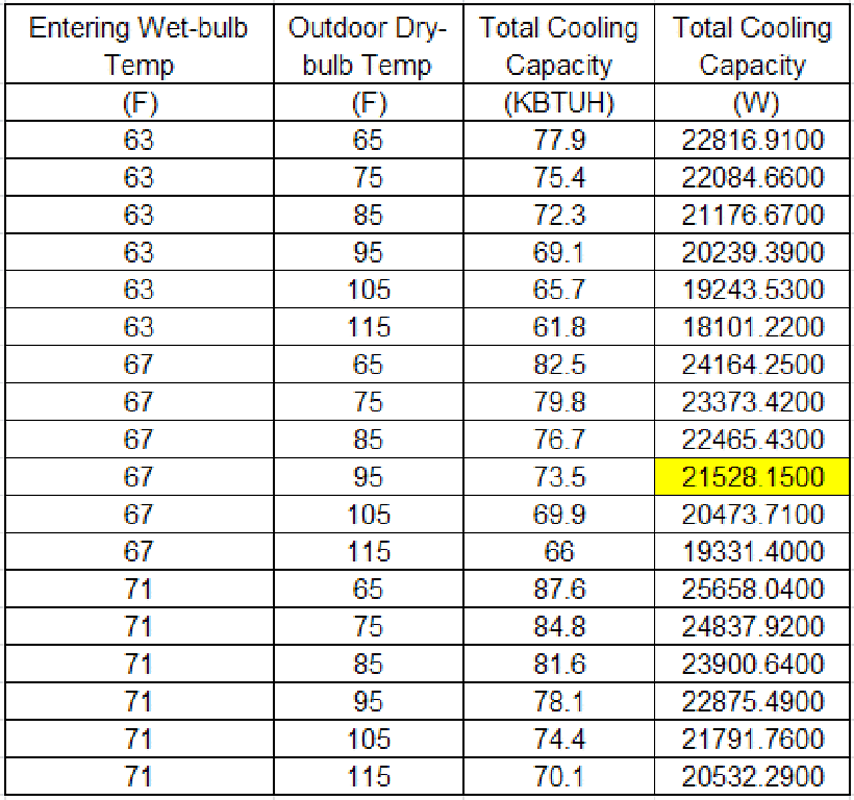
\includegraphics{media/image7865.png}
\caption{DataTable}
\end{figure}

The fundamental equation would be used to determine the number of independent variables and also the form of the equation. Given the example described here, the spreadsheet would be set up to look like the equation as shown in the following table. A regression analysis could then be performed on the data set. The first five columns are the independent variables and the last column is the dependent variable. A spreadsheet tool is selected to perform the regression analysis, and the coefficients are calculated and displayed in the spreadsheet.

\begin{figure}[htbp]
\centering
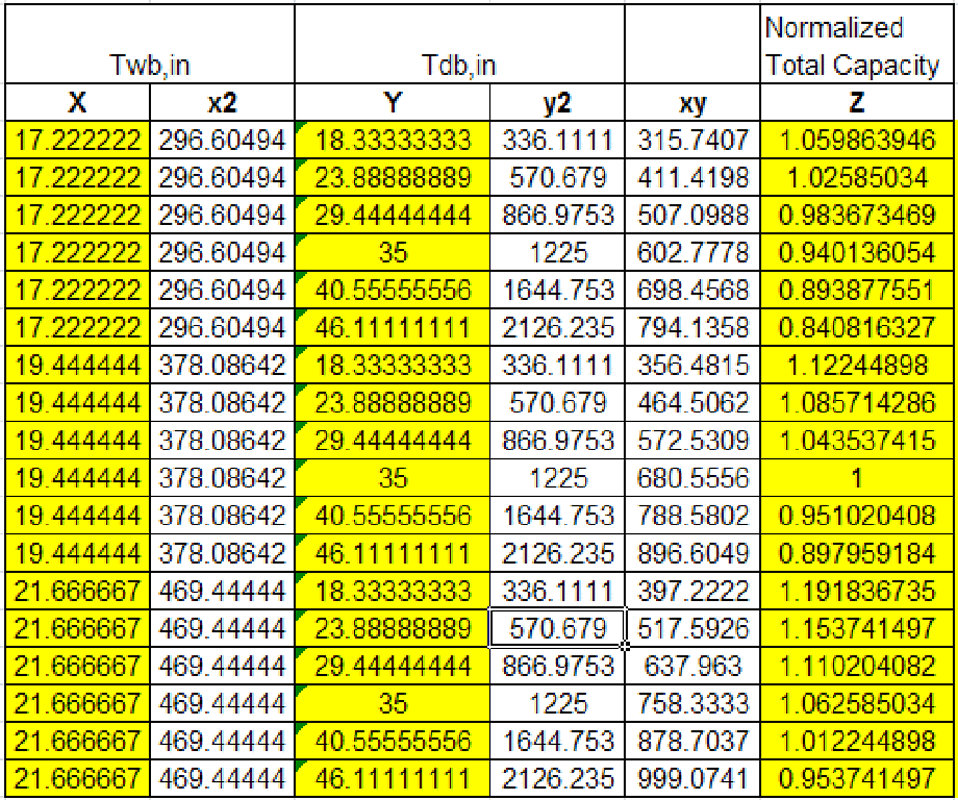
\includegraphics{media/image7866.png}
\caption{RegressionAnalysis}
\end{figure}

The regression analysis and summary statistical output is shown below. The equation coefficients are shown highlighted. In this example, the equation coefficents are: a = 0.757382, b = 0.014666, c = 0.000459, d = -0.00095, e = -6.7E-05, and f = -0.00015. These coefficients would be entered in a Curve:BiQuadratic object and used to describe the cooling capacity as a function of temperature for the DX cooling coil model. Minimum and Maximum values from the tabular data are entered as Min/Max values for the curve object. The values may be relaxed slightly with care to allow extrapolation as needed. A performance table may be used to automatically perform the regression analysis as described in the following section.

\begin{figure}[htbp]
\centering
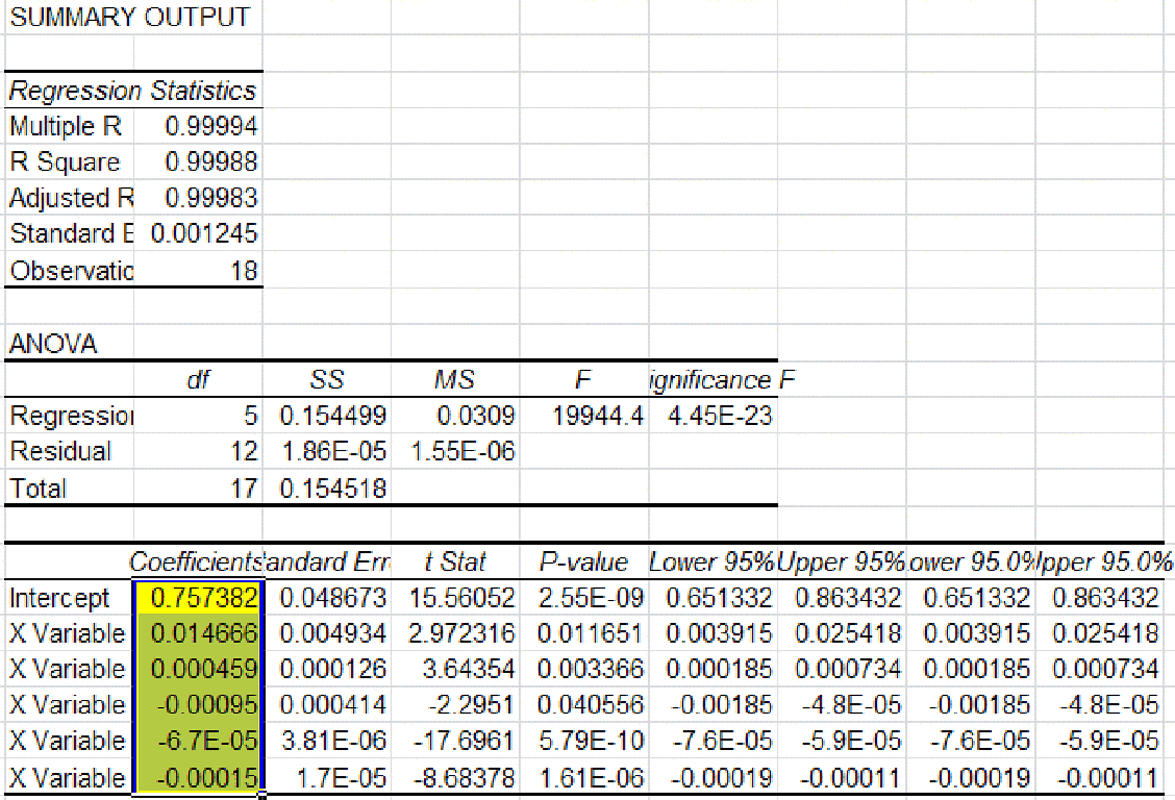
\includegraphics{media/image7867.png}
\caption{RegressionSummaryOutput}
\end{figure}

\begin{lstlisting}

  Curve:Biquadratic,
      CoolCapFTExample,        !- Name
      0.757382,                !- Coefficient1 Constant
      0.014666,                !- Coefficient2 x
      0.000459,                !- Coefficient3 x**2
      -0.00095,                !- Coefficient4 y
      -0.000067,               !- Coefficient5 y**2
      -0.00015,                !- Coefficient6 x*y
      17.22222,                !- Minimum Value of x
      21.66667,                !- Maximum Value of x
      18.33333,                !- Minimum Value of y
      46.11111,                !- Maximum Value of y
      ,                        !- Minimum Curve Output
      ,                        !- Maximum Curve Output
      Temperature,             !- Input Unit Type for X
      Temperature,             !- Input Unit Type for Y
      Dimensionless;           !- Output Unit Type
\end{lstlisting}

\subsection{Curves based on three independent variables}\label{curves-based-on-three-independent-variables}

A polynomial having three independent variables represents a three-dimensional relationship between a condition (the model inputs) and response (the model output).

\subsubsection{TriQuadratic Curves}\label{triquadratic-curves}

A performance curve having an order or degree of 2 in three independent variables.

\begin{equation}
\begin{array}{ll}
Output &= a + bx^2 + cx + dy^2 + ey + fz^2 + gz + hx^2y^2 + ixy + jxy^2 + kx^2y \\
       &+ lx^2z^2 + mxz + nxz^2 + ox^2z + py^2z^2 + qyz + ryz^2 + sy^2z + tx^2y^2z^2 \\
       &+ ux^2y^2z + ux^2yz^2 + vxy^2z^2 + wx^2yz + x\PB{xy^2z} + y\PB{xyz^2} + z\PB{xyz}
\end{array}
\end{equation}

\subsection{Pressure drop curve}\label{pressure-drop-curve}

\subsubsection{Functional Pressure Drop Curve}\label{functional-pressure-drop-curve}

A performance curve representing the minor loss and/or friction calculations in plant pressure simulations.

\begin{equation}
\Delta P = \left[ {K + f\left( {L/D} \right)} \right]\left( {\rho {V^2}} \right)/2
\end{equation}
